% Template to use to complete Problem Set 5.
% If you are using ShareLaTeX, you'll want to upload this file to your account.
% Before modifying this file, we recommend trying to compile it as-is
% to see what the basic template gives.

\documentclass[12pt]{article}
\usepackage{geometry}
\geometry{letterpaper}
\usepackage{amssymb}
\usepackage{amsmath}
\usepackage{graphicx, tikz}
\newcounter{ProblemNum}
\newcounter{SubProblemNum}[ProblemNum]
\renewcommand{\theProblemNum}{\arabic{ProblemNum}}
\renewcommand{\theSubProblemNum}{\alph{SubProblemNum}}
\newcommand*{\anyproblem}[1]{\newpage\subsection*{#1}}
\newcommand*{\problem}[1]{\stepcounter{ProblemNum} %
\anyproblem{Problem \theProblemNum. \; #1}}
\newcommand*{\soln}[1]{\subsubsection*{#1}}
\newcommand*{\solution}{\soln{Solution}}
\renewcommand*{\part}{\stepcounter{SubProblemNum} %
\soln{Part (\theSubProblemNum)}}


% Document metadata
\title{Problem Set \#5  \hspace{3cm} CSC236 Fall 2018}
\author{Mengning Yang, Chenxu Liu, Licheng Xu}
\date{December 6, 2018}


% Document starts here
\begin{document}
\maketitle



\noindent \rule{\textwidth}{1pt}





\vfill
We declare that this assignment is solely our own work, and is in accordance
with the University of Toronto Code of Behaviour on Academic Matters.

\noindent \rule{\textwidth}{1pt}

This submission has been prepared using \LaTeX.

\newpage
\problem{}
%%%%%%%%%%%%%%%
%%%%%%%%%%%%%%
\textsc{(Warmup - this problem will NOT be marked)}.
\\


For the following language, give an NFA that matches the language. Give informal justification for why your NFA is correct.

$L = \{w \in \{0,1\}^* \mid w \text{ starts with 01 but does not end with 01}\}$


%%Write your solution here

\problem{}
\textsc{(12 Marks)} Consider the following DFA for the language $L = \{ w \in \{0, 1\}^{*}$ $|$ $w$ begins with a 0 and ends with a 1\}, and answer the questions below. For each question, you should \textbf{only use the techniques that we covered in this course}.

\begin{center}
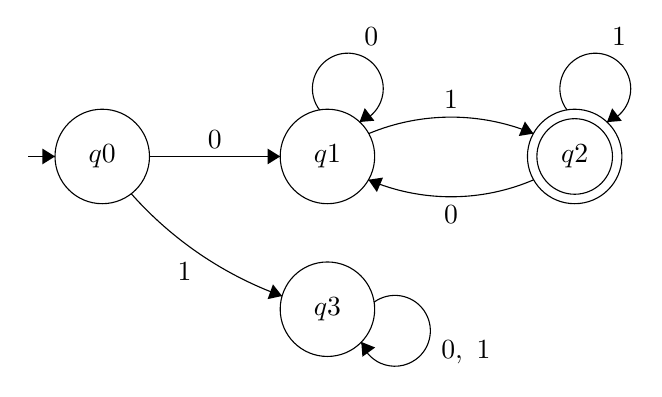
\begin{tikzpicture}[scale=0.2]
\tikzstyle{every node}+=[inner sep=0pt]
\draw [black] (17.8,-19.9) circle (3);
\draw (17.8,-19.9) node {$q0$};
\draw [black] (32.1,-19.9) circle (3);
\draw (32.1,-19.9) node {$q1$};
\draw [black] (47.8,-19.9) circle (3);
\draw (47.8,-19.9) node {$q2$};
\draw [black] (47.8,-19.9) circle (2.4);
\draw [black] (32.1,-29.6) circle (3);
\draw (32.1,-29.6) node {$q3$};
\draw [black] (13.1,-19.9) -- (14.8,-19.9);
\fill [black] (14.8,-19.9) -- (14,-19.4) -- (14,-20.4);
\draw [black] (20.8,-19.9) -- (29.1,-19.9);
\fill [black] (29.1,-19.9) -- (28.3,-19.4) -- (28.3,-20.4);
\draw (24.95,-19.4) node [above] {$0$};
\draw [black] (34.719,-18.449) arc (112.65484:67.34516:13.581);
\fill [black] (45.18,-18.45) -- (44.64,-17.68) -- (44.25,-18.6);
\draw (39.95,-16.9) node [above] {$1$};
\draw [black] (31.605,-16.953) arc (217.27542:-70.72458:2.25);
\draw (34.88,-12.89) node [above] {$0$};
\fill [black] (34.14,-17.71) -- (35.08,-17.63) -- (34.47,-16.83);
\draw [black] (29.221,-28.765) arc (-109.84827:-138.45152:23.431);
\fill [black] (29.22,-28.76) -- (28.64,-28.02) -- (28.3,-28.96);
\draw (23.02,-26.62) node [below] {$1$};
\draw [black] (45.199,-21.382) arc (-66.77953:-113.22047:13.313);
\fill [black] (34.7,-21.38) -- (35.24,-22.16) -- (35.63,-21.24);
\draw (39.95,-22.96) node [below] {$0$};
\draw [black] (47.315,-16.951) arc (217.07249:-70.92751:2.25);
\draw (50.61,-12.9) node [above] {$1$};
\fill [black] (49.85,-17.72) -- (50.79,-17.64) -- (50.18,-16.84);
\draw [black] (35.055,-29.157) arc (126.25533:-161.74467:2.25);
\draw (39.3,-32.32) node [right] {$0,\mbox{ }1$};
\fill [black] (34.25,-31.68) -- (34.32,-32.62) -- (35.13,-32.03);
\end{tikzpicture}
\end{center}

\begin{enumerate}
\item {(5 marks)} Prove that the DFA is correct (it matches exactly the language described above). Before beginning the proof, clearly state each of your \textbf{state invariants}.

\item {(2 Marks)}
Prove that this DFA has the minimal number of states (4 states).

\item {(5 Marks)} 
Using the \textbf{state elimination} method, convert the above DFA to its equivalent regular expression. You must show all your steps in \textbf{separate} figures.
\end{enumerate}
%%%%%%%%%%%%%%%%%%%%%%%%%%%%%%%%%%%%%%%%%%%%%%%%
%%%%%%%%%%%%%%problem 2 solution%%%%%%%%%%%%%%%%
%%%%%%%%%%%%%%%%%%%%%%%%%%%%%%%%%%%%%%%%%%%%%%%%
Answers:
\begin{enumerate}
\item
state invariants:\\
$q_0$ p(w):initial state, accepts empty strings\\
$q_1$ p(w):begins with 0,ends with 0\\
$q_2$ p(w):begins with 0, ends with 1\\
$q_3$ p(w):begins with 1\\

Base case:\\
Initial state is $q_0$, and $\epsilon$ is an empty string, so $\epsilon$ satisfies the invariant of $q_0$.\\
Base case holds.\\\\
Induction step: \\
We have seven transitions to check.\\
\uppercase\expandafter{\romannumeral1}: Assume some string w satisfies the invariant of $q_0$\\
if 0 transition is added which will give us w0 = 0, which satisfies the state invariant of $q_1$\\
if 1 transition is added which will give us w1= 1, which satisfies the state invariant of $q_3$\\\\
\uppercase\expandafter{\romannumeral2}: Assume some string w satisfies the invariant of $q_1$, then it must begin with 0.\\
if transition 1 is added, it will give us $w1 = 01$, which satisfies the state invariant of $q_2$\\
if transition 0 is added, then $w0 = 00$, satisfies the state invariant of $q_1$\\\\
\uppercase\expandafter{\romannumeral3}: Assume some string w satisfies the state invariant of $q_2$, then it must begin with 0 and ends with 1\\
if transition 0 is added, w0 now begins with 0 and ends with 0, so it goes back to $q_1$, and satisfies the state invariant of $q_1$\\
if transition 1 is added, w1 still begins with 0 and ends with 1, so it stays at $q_2$ and satisfies the state invariant of $q_2$\\\\
\uppercase\expandafter{\romannumeral4}: Assume some string w satisfies the state invariant of $q_3$, then it must begin with 1\\
if transition 1 and transition 0 is added, it will still give us a string that begins with 1, which satisfies the state invariant of $q_3$\\

Lastly, show that the state invariant of the accepting state exactly describe the languages that we want the DFA to accept. There is one accepting state which is $q_2$. If the string begins with 0 and ends with 1, it will satisfy the state invariant of $q_2$.\\
\item
Suppose for contradiction that we can find a correct DFA that has 3 states, then let\\
$w_{0}=\epsilon$\\
$w_{1}=1$\\
$w_{2}=0$\\
$w_{3}=01$\\
For one of the pairs of strings, the supposed 3-state DFA is forced into the same state for both strings (by the
Pigeonhole principle), and $w_ix$ and $w_jx$ must be both accepted or both rejected, for any string x. We will show, for each possible pair, that this is NOT true.\\\\

pair 1:\\
$w_{0}=\epsilon$ and $w_{1}=1$, $x=01$:\\
$w_{0}x=01$, accepted\\
$w_{1}x=101$, rejected\\
contradiction\\\\
pair 2:\\
$w_{0}=\epsilon$ and $w_{2}=0$, $x=1$:\\
$w_{0}x=1$, rejected\\
$w_{2}x=01$, accepted\\
contradiction\\\\
pair 3:\\
$w_{0}=\epsilon$ and $w_{3}=01$:\\
no need to choose an x\\
$w_{0}$ is rejected\\
$w_{3}$ is accepted\\
contradiction\\\\
pair 4:\\
$w_{1}=1$ and $w_{2}=0$, $x=1$:\\
$w_{1}x=11$, rejected\\
$w_{2}x=01$, accepted\\
contradiction\\\\
pair 5:\\
$w_{1}=1$ and $w_{3}=01$:\\
no need to choose an x\\
$w_{1}$ is rejected\\
$w_{3}$ is accepted\\
contradiction\\\\
pair 6:\\
$w_{2}=0$ and $w_{3}=01$:\\
no need to choose an x\\
$w_{2}$ is rejected\\
$w_{3}$ is accepted\\
contradiction\\\\
$\therefore$ None of these pairs is both accepted nor rejected.\\
$\therefore$ There are at least 4 states.\\


3.\\
\begin{center}
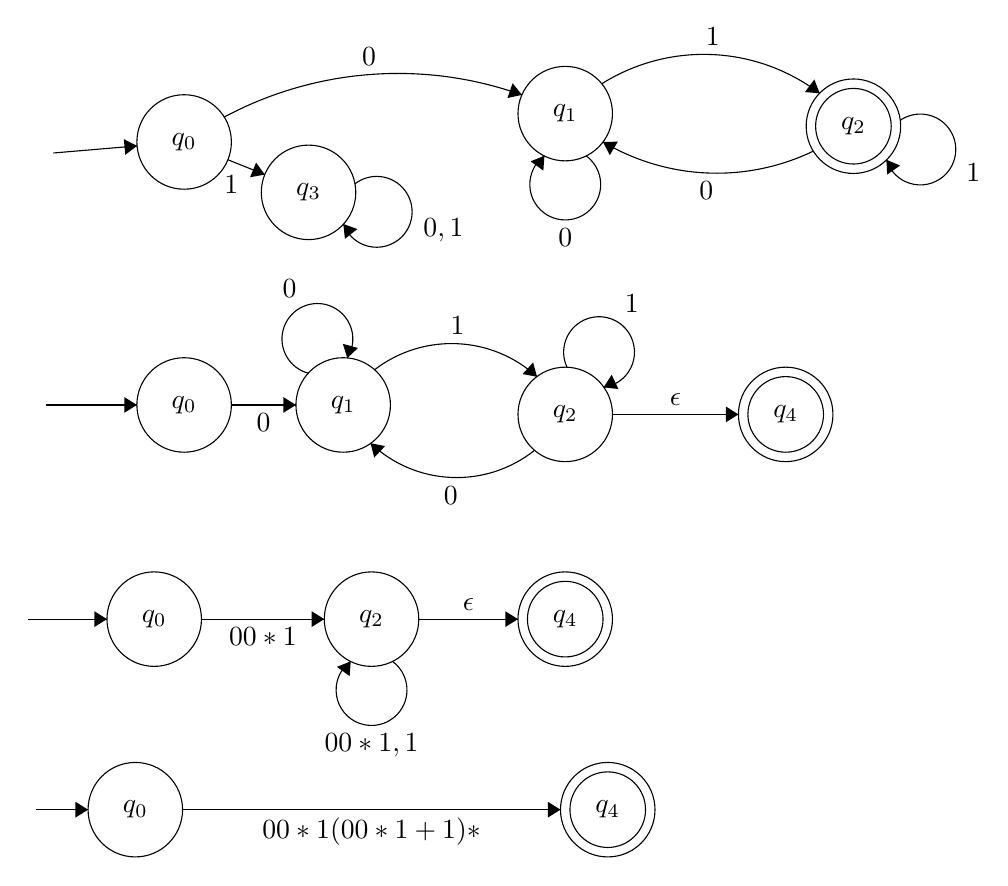
\begin{tikzpicture}[scale=0.2]
\tikzstyle{every node}+=[inner sep=0pt]
\draw [black] (10.3,-26) circle (3);
\draw (10.3,-26) node {$q_0$};
\draw [black] (20.4,-26) circle (3);
\draw (20.4,-26) node {$q_1$};
\draw [black] (34.5,-26.6) circle (3);
\draw (34.5,-26.6) node {$q_2$};
\draw [black] (48.5,-26.6) circle (3);
\draw (48.5,-26.6) node {$q_4$};
\draw [black] (48.5,-26.6) circle (2.4);
\draw [black] (10.3,-9.3) circle (3);
\draw (10.3,-9.3) node {$q_0$};
\draw [black] (18.2,-12.5) circle (3);
\draw (18.2,-12.5) node {$q_3$};
\draw [black] (34.5,-7.5) circle (3);
\draw (34.5,-7.5) node {$q_1$};
\draw [black] (52.8,-8.3) circle (3);
\draw (52.8,-8.3) node {$q_2$};
\draw [black] (52.8,-8.3) circle (2.4);
\draw [black] (8.4,-39.6) circle (3);
\draw (8.4,-39.6) node {$q_0$};
\draw [black] (22.2,-39.6) circle (3);
\draw (22.2,-39.6) node {$q_2$};
\draw [black] (34.5,-39.6) circle (3);
\draw (34.5,-39.6) node {$q_4$};
\draw [black] (34.5,-39.6) circle (2.4);
\draw [black] (7.2,-51.7) circle (3);
\draw (7.2,-51.7) node {$q_0$};
\draw [black] (37.2,-51.7) circle (3);
\draw (37.2,-51.7) node {$q_4$};
\draw [black] (37.2,-51.7) circle (2.4);
\draw [black] (22.383,-23.772) arc (127.62698:47.49973:8.032);
\fill [black] (32.71,-24.21) -- (32.46,-23.3) -- (31.79,-24.04);
\draw (27.67,-21.57) node [above] {$1$};
\draw [black] (13.3,-26) -- (17.4,-26);
\fill [black] (17.4,-26) -- (16.6,-25.5) -- (16.6,-26.5);
\draw (15.35,-26.5) node [below] {$0$};
\draw [black] (1.5,-26) -- (7.3,-26);
\fill [black] (7.3,-26) -- (6.5,-25.5) -- (6.5,-26.5);
\draw [black] (18.193,-23.985) arc (255.33155:-32.66845:2.25);
\draw (17,-19.19) node [above] {$0$};
\fill [black] (20.66,-23.02) -- (21.34,-22.38) -- (20.38,-22.12);
\draw [black] (32.565,-28.869) arc (-51.29725:-133.57605:7.933);
\fill [black] (22.14,-28.43) -- (22.37,-29.34) -- (23.06,-28.61);
\draw (27.23,-31.14) node [below] {$0$};
\draw [black] (34.618,-23.614) arc (205.46387:-82.53613:2.25);
\draw (38.72,-20.17) node [above] {$1$};
\fill [black] (36.94,-24.88) -- (37.88,-24.99) -- (37.45,-24.08);
\draw [black] (37.5,-26.6) -- (45.5,-26.6);
\fill [black] (45.5,-26.6) -- (44.7,-26.1) -- (44.7,-27.1);
\draw (41.5,-26.1) node [above] {$\epsilon$};
\draw [black] (2,-10) -- (7.31,-9.55);
\fill [black] (7.31,-9.55) -- (6.47,-9.12) -- (6.56,-10.12);
\draw [black] (12.846,-7.718) arc (118.18175:70.32593:23.366);
\fill [black] (31.75,-6.31) -- (31.16,-5.57) -- (30.83,-6.51);
\draw (22.04,-4.45) node [above] {$0$};
\draw [black] (13.08,-10.43) -- (15.42,-11.37);
\fill [black] (15.42,-11.37) -- (14.87,-10.61) -- (14.49,-11.54);
\draw (13.29,-11.42) node [below] {$1$};
\draw [black] (21.14,-11.965) arc (128.0546:-159.9454:2.25);
\draw (25.46,-14.92) node [right] {$0,1$};
\fill [black] (20.41,-14.51) -- (20.51,-15.45) -- (21.3,-14.83);
\draw [black] (36.817,-5.607) arc (122.18413:52.80959:12.17);
\fill [black] (50.66,-6.21) -- (50.32,-5.33) -- (49.72,-6.13);
\draw (43.87,-3.21) node [above] {$1$};
\draw [black] (50.257,-9.88) arc (-64.23399:-120.77229:14.119);
\fill [black] (36.9,-9.3) -- (37.33,-10.14) -- (37.84,-9.28);
\draw (43.46,-11.81) node [below] {$0$};
\draw [black] (55.765,-7.931) arc (124.82099:-163.17901:2.25);
\draw (59.94,-11.26) node [right] {$1$};
\fill [black] (54.9,-10.43) -- (54.94,-11.37) -- (55.76,-10.8);
\draw [black] (0.4,-39.6) -- (5.4,-39.6);
\fill [black] (5.4,-39.6) -- (4.6,-39.1) -- (4.6,-40.1);
\draw [black] (11.4,-39.6) -- (19.2,-39.6);
\fill [black] (19.2,-39.6) -- (18.4,-39.1) -- (18.4,-40.1);
\draw (15.3,-40.1) node [below] {$00*1$};
\draw [black] (25.2,-39.6) -- (31.5,-39.6);
\fill [black] (31.5,-39.6) -- (30.7,-39.1) -- (30.7,-40.1);
\draw (28.35,-39.1) node [above] {$\epsilon$};
\draw [black] (23.523,-42.28) arc (54:-234:2.25);
\draw (22.2,-46.85) node [below] {$00*1,1$};
\fill [black] (20.88,-42.28) -- (20,-42.63) -- (20.81,-43.22);
\draw [black] (0.9,-51.7) -- (4.2,-51.7);
\fill [black] (4.2,-51.7) -- (3.4,-51.2) -- (3.4,-52.2);
\draw [black] (10.2,-51.7) -- (34.2,-51.7);
\fill [black] (34.2,-51.7) -- (33.4,-51.2) -- (33.4,-52.2);
\draw (22.2,-52.2) node [below] {$00*1(00*1+1)*$};
\draw [black] (35.823,-10.18) arc (54:-234:2.25);
\draw (34.5,-14.75) node [below] {$0$};
\fill [black] (33.18,-10.18) -- (32.3,-10.53) -- (33.11,-11.12);
\end{tikzpicture}
\end{center}
\end{enumerate}
%%%%%%%%%%%%%%%%%%%%%%%%%%%%%%%%%%%%%%%%%%%%%%%%
%%%%%%%%%%%%%%%%%%%%%%%%%%%%%%%%%%%%%%%%%%%%%%%%
%%%%%%%%%%%%%%%%%%%%%%%%%%%%%%%%%%%%%%%%%%%%%%%%
\problem{}
\textsc{(4 Marks)} Use the subset construction algorithm from lecture to produce an equivalent DFA from the following NFA. Please show your work so that we know how each state is generated. Name your DFA states so that the link to the NFA states is clear; i.e.\, you should have DFA states that look like $\{q_0, q_1\}$.

\begin{tabular}{ccc}
Old State & Symbol & New State \\
\hline
$q_0$ & 0 & $q_2$ \\
$q_0$ & 0 & $q_3$ \\
$q_0$ & 1 & $q_1$ \\
$q_0$ & 1 & $q_4$ \\
$q_1$ & 0 & $q_2$ \\
$q_1$ & 1 & $q_1$ \\
$q_2$ & 0 & $q_1$ \\
$q_2$ & 1 & $q_2$ \\
$q_3$ & 0 & $q_3$ \\
$q_3$ & 1 & $q_4$ \\
$q_4$ & 0 & $q_4$ \\
$q_4$ & 1 & $q_5$ \\
$q_5$ & 0 & $q_5$
\end{tabular}

The start state of this NFA is $q_0$; the accepting (final) states are $q_0$, $q_1$, and $q_5$.\\\\
  
%%Write your solution here
\noindent Answer:\\
\noindent\{$q_0$\}--$\epsilon$--\{$q_0$\}(initial state of the DFA)\\
\{$q_0$\}--$0$--\{$q_2$,$q_3$\}(new state!)\\
\{$q_0$\}--$1$--\{$q_1$,$q_4$\}(new state!)\\
\{$q_2$,$q_3$\}--$0$--\{$q_1$,$q_3$\}(new state!)\\
\{$q_2$,$q_3$\}--$1$--\{$q_2$,$q_4$\}(new state!)\\
\{$q_1$,$q_4$\}--$0$--\{$q_2$,$q_4$\}\\
\{$q_1$,$q_4$\}--$1$--\{$q_1$,$q_5$\}(new state!)\\
\{$q_1$,$q_3$\}--$0$--\{$q_2$,$q_3$\}\\
\{$q_1$,$q_3$\}--$1$--\{$q_1$,$q_4$\}\\
\{$q_2$,$q_4$\}--$0$--\{$q_1$,$q_4$\}\\
\{$q_2$,$q_4$\}--$1$--\{$q_2$,$q_5$\}(new state!)\\
\{$q_1$,$q_5$\}--$0$--\{$q_2$,$q_5$\}\\
\{$q_1$,$q_5$\}--$1$--\{$q_1$\}(new state!)\\
\{$q_2$,$q_5$\}--$0$--\{$q_1$,$q_5$\}\\
\{$q_2$,$q_5$\}--$1$--\{$q_2$\}(new state!)\\
\{$q_1$\}--$0$--\{$q_2$\}\\
\{$q_1$\}--$1$--\{$q_1$\}\\
\{$q_2$\}--$0$--\{$q_1$\}\\
\{$q_2$\}--$1$--\{$q_2$\}\\


\begin{center}
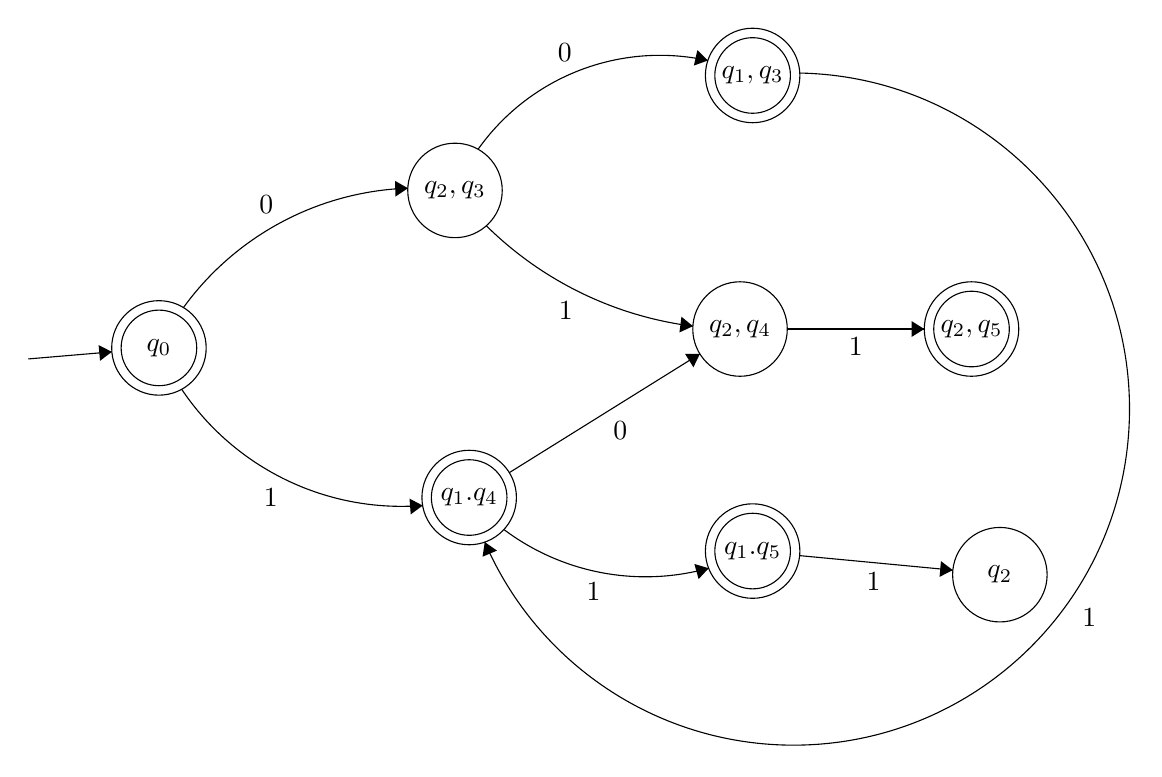
\begin{tikzpicture}[scale=0.2]
\tikzstyle{every node}+=[inner sep=0pt]
\draw [black] (9.5,-28.5) circle (3);
\draw (9.5,-28.5) node {$q_0$};
\draw [black] (9.5,-28.5) circle (2.4);
\draw [black] (29.2,-38) circle (3);
\draw (29.2,-38) node {${q_1.q_4}$};
\draw [black] (29.2,-38) circle (2.4);
\draw [black] (28.3,-18.5) circle (3);
\draw (28.3,-18.5) node {${q_2,q_3}$};
\draw [black] (46.4,-27.3) circle (3);
\draw (46.4,-27.3) node {${q_2,q_4}$};
\draw [black] (47.2,-11.2) circle (3);
\draw (47.2,-11.2) node {${q_1,q_3}$};
\draw [black] (47.2,-11.2) circle (2.4);
\draw [black] (61.1,-27.3) circle (3);
\draw (61.1,-27.3) node {${q_2,q_5}$};
\draw [black] (61.1,-27.3) circle (2.4);
\draw [black] (47.2,-41.4) circle (3);
\draw (47.2,-41.4) node {${q_1.q_5}$};
\draw [black] (47.2,-41.4) circle (2.4);
\draw [black] (62.9,-42.9) circle (3);
\draw (62.9,-42.9) node {${q_2}$};
\draw [black] (1.2,-29.2) -- (6.51,-28.75);
\fill [black] (6.51,-28.75) -- (5.67,-28.32) -- (5.76,-29.32);
\draw [black] (11.056,-25.939) arc (144.05034:91.96802:18.384);
\fill [black] (25.31,-18.36) -- (24.49,-17.89) -- (24.52,-18.89);
\draw (16.31,-20) node [above] {$0$};
\draw [black] (26.247,-38.506) arc (-85.38658:-146.10326:16.809);
\fill [black] (26.25,-38.51) -- (25.41,-38.07) -- (25.49,-39.07);
\draw (16.61,-37.4) node [below] {$1$};
\draw [black] (43.408,-27.121) arc (-97.20742:-134.64949:22.724);
\fill [black] (43.41,-27.12) -- (42.68,-26.52) -- (42.55,-27.52);
\draw (35.33,-25.52) node [below] {$1$};
\draw [black] (29.764,-15.888) arc (144.65297:77.58448:14.161);
\fill [black] (44.36,-10.25) -- (43.69,-9.59) -- (43.47,-10.57);
\draw (35.27,-10.35) node [above] {$0$};
\draw [black] (49.4,-27.3) -- (58.1,-27.3);
\fill [black] (58.1,-27.3) -- (57.3,-26.8) -- (57.3,-27.8);
\draw (53.75,-27.8) node [below] {$1$};
\draw [black] (44.409,-42.487) arc (-74.46837:-126.92465:14.975);
\fill [black] (44.41,-42.49) -- (43.5,-42.22) -- (43.77,-43.18);
\draw (37.1,-43.36) node [below] {$1$};
\draw [black] (31.75,-36.42) -- (43.85,-28.88);
\fill [black] (43.85,-28.88) -- (42.91,-28.88) -- (43.44,-29.73);
\draw (38.8,-33.15) node [below] {$0$};
\draw [black] (50.19,-41.69) -- (59.91,-42.61);
\fill [black] (59.91,-42.61) -- (59.16,-42.04) -- (59.07,-43.04);
\draw (54.88,-42.73) node [below] {$1$};
\draw [black] (50.194,-11.046) arc (88.91588:-156.6898:21.342);
\fill [black] (30.19,-40.83) -- (30.05,-41.76) -- (30.97,-41.37);
\draw (68.11,-45.62) node [right] {$1$};
\end{tikzpicture}
\end{center}
\end{document}